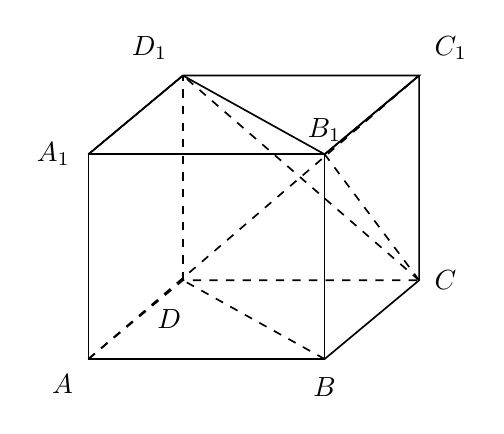
\begin{tikzpicture}[line width=0.6pt, >=stealth]
\coordinate (A) at (0,0);
\coordinate (B) at (3.0,0);
\coordinate (C) at (4.2,1.0);
\coordinate (D) at (1.2,1.0);
\coordinate (Aone) at (0,2.6);
\coordinate (Bone) at (3.0,2.6);
\coordinate (Cone) at (4.2,3.6);
\coordinate (Done) at (1.2,3.6);
% solid outer cube
\draw (A) -- (B) -- (Bone) -- (Aone) -- cycle;
\draw (Aone) -- (Done) -- (Cone) -- (Bone);
\draw (Bone) -- (Cone);
\draw (Done) -- (Cone);
\draw (Cone) -- (C) -- (B);
\draw (Done) -- (Aone);
\draw (Aone) -- (Bone);
% top triangle edge B1-D1
\draw (Bone) -- (Done);
% hidden cube edges
\draw[dashed] (A) -- (D) -- (C);
\draw[dashed] (D) -- (Done);
% bottom diagonal BD hidden
\draw[dashed] (B) -- (D);
% body diagonal AC1
\draw[dashed] (A) -- (Cone);
% triangle CB1D1
\draw[dashed] (C) -- (Bone);
\draw[dashed] (C) -- (Done);
% labels
\node[below left=2pt] at (A) {$A$};
\node[below=3pt] at (B) {$B$};
\node[right=2pt] at (C) {$C$};
\node[below left=2pt,xshift=5pt,yshift=-5pt] at (D) {$D$};
\node[left=3pt] at (Aone) {$A_{1}$};
\node[above=1pt] at (Bone) {$B_{1}$};
\node[above right=2pt] at (Cone) {$C_{1}$};
\node[above left=2pt] at (Done) {$D_{1}$};
\end{tikzpicture}
